O pr�ximo teste (Tabela \ref{tabela:teste2}) mostra o impacto variando o n�mero de terrenos vizinhos. Como era de se esperar, quanto maior o n�mero de vizinhos, menor o FPS. Para melhorar isso, � poss�vel ajustar o n�mero de vizinhos desenhados de acordo com o computador.

\begin{table}[H]
	\begin{center}
		\begin{tabular}{|c|c|c|c|c|}
			\hline
			 - & \multicolumn{3}{|c|}{\emph{Frames} por segundo} \\
			\hline
			Vizinhos & \scriptsize M�n. & \scriptsize M�x. & \scriptsize M�dia \\
			\hline
			2 & 17,0 & 75,0 & 38,5 \\
			\hline
			4 & 4,0 & 20,0 & 15,8 \\
			\hline
			8 & 0 & 5,0 & 4,1 \\
			\hline
		\end{tabular}
		\caption{FPS das execu��es variando o n�mero de terrenos vizinhos, e o n�mero de octaves fixo.}
		\label{tabela:teste2}
	\end{center}
\end{table}

%\begin{figure}[H]
	%\center{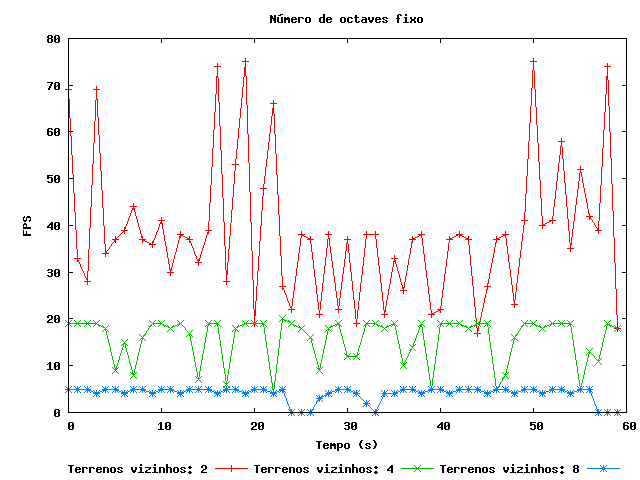
\includegraphics[width=0.8\linewidth]{img/graficos/teste2/teste2.png}}
	%\caption{\label{fig:teste2} Teste variando o n�mero de terrenos vizinhos, e o n�mero de octaves fixo.}
%\end{figure}